\documentclass[12pt]{article}

\usepackage{graphicx}
\graphicspath{ {./images/} }

\begin{document}

\title{Activity VI: Planetary Systems}

\maketitle

Answer the following open-ended questions about the planets.
\begin{enumerate}
        \item In Figure 1, we have multiple objects which orbit various axes.
            \begin{enumerate}
              \item List (e), (f), and (g) in ascending order of their moments of inertia. Assume they all have the same mass.
                    \begin{enumerate}
                        \item (f) has the least moment of inertia as there is no separation of mass from the center of rotation.
                        \item (e) has the next least moment of inertia as the mass is separated from the center of rotation. However, this distance is not as much as (g).
                        \item (g) has the most moment of inertia because all the mass is concentrated around the edge of the cylinder and has the greatest separation from the center of rotation.
                    \end{enumerate}
              \item Between (h) and (i), which one has a greater moment of inertia? Assume they have the same mass.\newline\newline
                    (i) has the greater moment of inertia because it's mass is focused at the edge of the sphere which means it's separated from the center of rotation.

              \item In (g), we have a hollow cylinder of radius R. Suppose that its radius shrinks by one-half. Will its moment of inertia increase or decrease, or will it stay the same? If it rotates at 3.0 revolutions per second with a radius R, will it rotate faster or slower than 3.0 revolutions per second if its radius decreases by one-half? Explain via the conservation of angular momentum.\newline\newline
                    Assuming the mass still stays the same, after the radius shrinks by one-half, the moment of inertia will decrease because the mass is closer to the center of rotation (there is less separation).\newline

                    Assuming the mass stays the same, it will rotate faster because of the conservation of angular velocity. Which basically states moment of inertia times angular velocity must be equal to some constant.\newline

                    moment of inertia $\times$ angular velocity = constant\newline

                    This means that if the moment of inertia decreases then the angular velocity must inecrase and vice versa. Therefore if the radius is halved, the object will rotate faster.

              \item Suppose that the moment of inertia of a protoplanetary disk doubles. If its initial angular velocity is $2\pi$ radians/second, how fast will it rotate after its moment of inertia changes?\newline\newline
                    Since the moment of inertia and the angular velocity must be proportional to some constant. The factor by which one increases must be the factor by with the other decreases.\newline

                    Therefore if the moment of inertia doubles, then the angular velocity must be halved.\newline

                    Angular velocity after: \newline
                    \centerline{$\frac{2\pi}{2} = \pi  $ rad/s}


            \end{enumerate}
        \item An ant walks 2.0 m around a circle of radius 1.0 m. Through what angle
        did the ant walk? State your answer in degrees.\newline

        Arc length = 2m\newline
        Radius = 1m

        \begin{equation}
          \theta = \frac{L}{r} = \frac{2}{1} =  2 \textnormal{ rad} = 114.6^{\circ}
        \end{equation}

        \item Suppose there is a planetary system consisting of one star and two exoplanets which orbit in circular orbits. The second exoplanet orbits at twice the distance of the first exoplanet. How much more light does the first exoplanet get compared to the second one? State your answer in terms of a ratio.\newline

        \begin{equation}
        Intensity = \frac{1}{d^{2}}
        \end{equation}

        Let f be the distance from the star to the first planet\newline

        \begin{equation}
        Intensity = \frac{1}{f^{2}}
        \end{equation}

        Therfore the intensity of light at the second planet should be:
        \begin{equation}
        Intensity = \frac{1}{(2f)^{2}}
        \end{equation}

        Now let's put the intensity of both planets into a ratio:

        \begin{equation}
            r = \frac{\frac{1}{f^{2}}}{\frac{1}{(2f)^{2}}}
        \end{equation}

        \begin{equation}
            r = \frac{1}{f^{2}} \times \frac{(2f)^{2}}{1}
        \end{equation}

        \begin{equation}
            r = \frac{1}{f^{2}} \times \frac{4f^{2}}{1}
        \end{equation}

        \begin{equation}
            r = 4
        \end{equation}

        Therefore, the second planet receives 0.25 of the amount of light the first planet receives.


        \begin{center}
        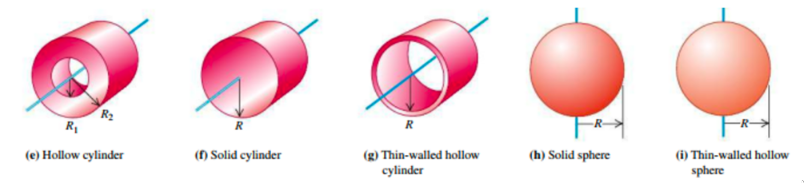
\includegraphics[scale=0.55]{a6f1}

        Figure 1: This figure shows objects of various moments of inertia.
        \end{center}


        \item Mars gets about $43\%$ of the light that the Earth gets. Approximately how much farther does Mars orbit from the Sun than does the Earth? Compare your answer to the literature value.\newline

        According to the inverse square law, the amount of light a planet receives is inversely proportional to the distance from star squared.\newline

        Distance from sun:

        \begin{equation}
            0.43 = \frac{1}{d^{2}}
        \end{equation}

        \begin{equation}
            0.43\times d^{2} = 1
        \end{equation}

        \begin{equation}
            d^{2} = \frac{1}{0.43}
        \end{equation}

        \begin{equation}
            d^{2} = 2.325
        \end{equation}

        \begin{equation}
            d = 1.54
        \end{equation}

        Mars orbits the sun at about 1.54 AU and the earth orbits the sun at about 1 AU. Which means mars orbits the sun 0.54 AU farther than earth.

        \item Which of the following facts, if true, would not be easily explainable via the nebular hypothesis? Select all that apply.
        \begin{enumerate}
            \item The planets have randomly distributed eccentricities.\newline
                This could be explained via nebular hypothesis.
            \item The planets orbit in the same plane.\newline
                This cannot be easily explained via nebular hypothesis.
            \item The iciest SSBs are closer to the sun.\newline
                This can be proved by nebular hypothesis.
            \item Most meteorites are about 7 billion years old.\newline
                This could be explained via nebular hypothesis.
        \end{enumerate}
        \item Give three reasons why Pluto should be considered a dwarf planet in the Kuiper Belt, as opposed to a planet.
            \begin{enumerate}
                \item Pluto is very small compared to other planets in the solar system
                \item Pluto overlaps it's orbit with other planets
                \item Pluto has objects on its orbital path around the sun whereas planets have a clear orbital path
            \end{enumerate}
        \item TRAPPIST-1e has a mass about 0.77 that of Earth, and a radius 0.91 that of Earth. Compute the surface gravity on the planet.\newline

        TRAPPIST-1e mass: $4.598594\times10^{24}$ kg\newline
        TRAPPIST-1e radius: 5804071 m


        \begin{equation}
          g = \frac{(6.67 \times 10^{-11})\times(4.598594\times10^{24})}{(5804071)^{2}}
        \end{equation}

        \begin{equation}
          g = \frac{3.06726219\times10^{14}}{(5804071)^{2}}
        \end{equation}

        \begin{equation}
          g = 9.10511568 \textnormal{ m/s}^{2}
        \end{equation}

\end{enumerate}
————————————————

\end{document}
